\documentclass[12pt]{article}

\usepackage{graphicx}
\usepackage{listings}
\usepackage{url}


\title{Project Assignment\\
Parallel Solver for Traveling Salesman Problem}
\author{Massimo Di Pierro}

\begin{document}

\maketitle

Your project consists of implementing a parallel solver for the
Traveling Salesman Problem and writing a short paper to document your
solution.

The deadline for the project is Sat Feb 9, 2013.

\begin{center}
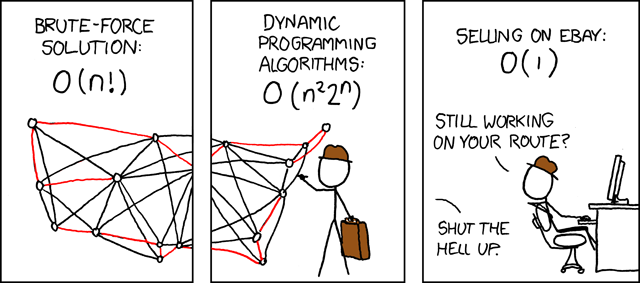
\includegraphics[width=4in]{travelling.png}
\end{center}

\section{Requirements about Code}

\begin{itemize}
\item Your code must be written in C/C++ with MPI and/or in Python
  with {\tt psim.py}.
\item It is recommended that you implement a parallel version  of the Branch-Bound algorithm. You can use the Held-Karp which is faster but also more difficult to implement.
\item The algorithm must take as input a flat text file of the CSV form:
\begin{lstlisting}
0, 1, 10.9628629098
0, 3, 8.98886303215
0, 4, 6.65365965779
1, 2, 4.52195982628
1, 3, 1.70565185304
2, 3, 3.32596142881
2, 4, 4.23563784771
\end{lstlisting}
where the first and second column are indices of the vertices (from 0 to N-1) and the third column is the distance between vertices. The program should read the input, parse it, determine the total number of vertices, and build a representation of the graph. Some links may be missing from the file, this means the corresponding distance is infinity. The order of the links in the input file is not specified.
\item The program should output the shortest path that visits all vertices and returns to the origin. This should be in the form of flat file containing a list of indices of vertices in the order in which they are visited, separated by a comma. The traveling salesman always start at vertex 0 (origin). For example
\begin{lstlisting}
0, 4, 2, 3, 1
\end{lstlisting}
\item The program should  run (20 points)
\item The program should return the correct result (10)
\item Each function must include a documentation comment including
  description of input, output, and purpose for the function. (3)
\item Each call to communication functions must include a comment
  explaining what data is communicated. (3)
\item The program should not contain memory leaks. (2)
\item The program must be properly indented. (1)
\item The program should not contain un-necessary code nor commented
  code. (1)
\item Compact code is better than verbose code.
\end{itemize}

\section{Requirements about Documentation}

The documentation should be in the form of paper containing:

\begin{itemize}
\item An introduction (no formulas or code) (2 points)
\item Examples of applications (2 points)
\item A description of the non-parallel algorithm with pseudocode and
  discussion of running time (2 points)
\item An overview of existing parellel implementations. (2 points)
\item A description of your data representation. (2 points)
\item A description of the parallel algorithm that you used (2 points)
\item A description of your implementation of the algorithm (2 points)
\item Formulas for Speedup, Efficiency, and Cost in the best case and
  in the worst case. (6 points)
\item Benchmarks for your algorithm for one, two and four parallel
  processes (even if you run it on a single node and therefore does
  not scale). (2 points)
\item List of references to papers you found useful or quoted.
\item Appendices with your code (both serial and parallel).
\end{itemize}

The total length of the paper excluding the appendices with program
should be more then 10 pages long and less then 30.

\begin{thebibliography}{999}

\bibitem{tsp1}
\url{https://wiki.engr.illinois.edu/download/attachments/203953697/report-TSP.pdf}

\bibitem{gputsp}
\url{http://arxiv.org/pdf/1208.3933.pdf}

\bibitem{applications}
\url{http://arxiv.org/pdf/1208.3933.pdf}

\bibitem{steps}
\url{http://www.jot.fm/issues/issue_2003_03/column7.pdf}
\url{http://www.jot.fm/issues/issue_2003_05/column7.pdf}
\url{http://www.jot.fm/issues/issue_2003_07/column8.pdf}
\url{http://www.jot.fm/issues/issue_2003_11/column5.pdf}
\end{thebibliography}


\end{document}
